\documentclass[12pt, a4paper]{article}
\usepackage[affil-it]{authblk} 
\usepackage{etoolbox}
\usepackage{lmodern}
\usepackage{titlesec}
\usepackage{enumitem}
\usepackage{float}
\usepackage{amsmath}
\usepackage{mathtools}
\makeatletter
\patchcmd{\@maketitle}{\LARGE \@title}{\fontsize{20}{19.2}\selectfont\@title}{}{}
\makeatother

\renewcommand\Authfont{\fontsize{16}{14.4}\selectfont}
\renewcommand\Affilfont{\fontsize{12}{10.8}\itshape}

\title{\textbf{Inverted Pendulum}} 
\author{Group 12}
\usepackage{graphicx}
\begin{document}
\maketitle
\newpage
\tableofcontents
\newpage
\section{Introduction}
\begin{figure}[H]
\centering
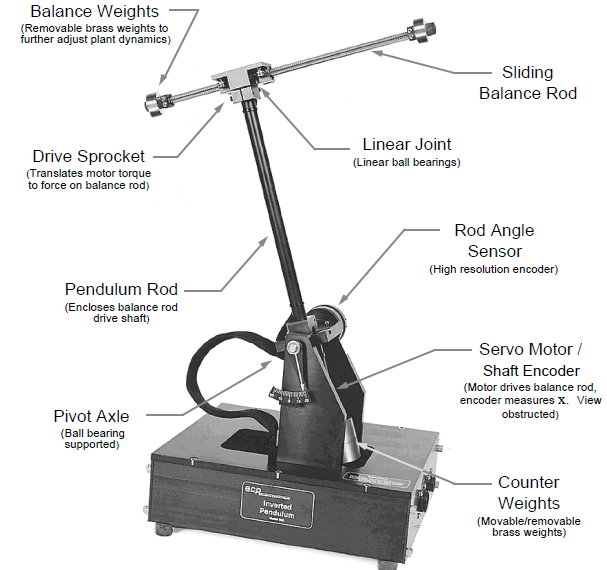
\includegraphics[width = \textwidth]{pendulumfoto.png}
\caption{Inverted Pendulum with sliding rod}
\label{Fig1}
\end{figure}
An inverted pendulum is a pendulum that has its center of mass above its pivot point.It steers a horizontal sliding rod in the presence of gravity to balance and control the position of the vertical rod(pendulum). The mechanism is open-loop unstable (right half plane pole) and non-minimum phase (right half plane zero). Hence a feedback control is essential for the stability and the structure of the controller must be selected carefully because of the non-minimum phase characteristic.
\begin{figure}[H]
\centering
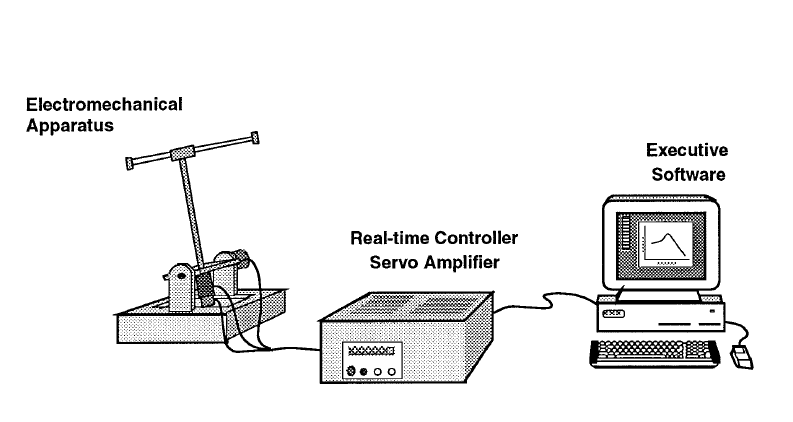
\includegraphics[width = \textwidth]{system.png}
\caption{Experimental Control System}
\label{Fig2}
\end{figure}
The experimental control system is comprised of three subsystems shown in figure \ref{Fig2}. The electromechanical plant consists of the inverted pendulum, its actuators and sensors. The design features a DC servo motor, high resolution encoders, a low friction sliding balance rod and adjustable weight balance. The real time controller servo amplifier unit contains a digital signal processor based real time controller, servo actuators, servo amplifiers and auxiliary power supplies. The executive program runs on a PC in MS DOS. This menu driven program is the user’s interface to the system and supports controller specification, trajectory definition, data acquisition, plotting etc.
\section{Plant Model}
\begin{figure}[H]
\centering
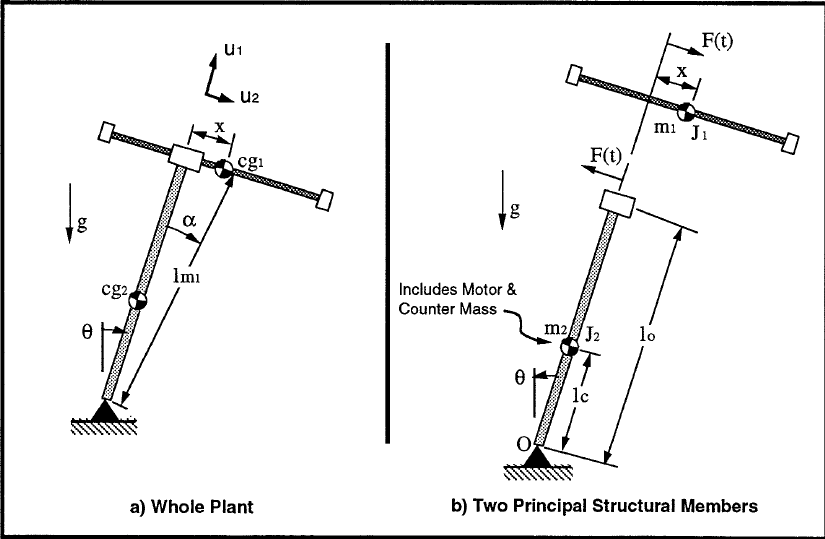
\includegraphics[width = \textwidth]{plant_model.png}
\caption{Plant Model}
\label{Fig3}
\end{figure}
The figure \ref{Fig3} shows the model of the pendulum-rod assembly. The friction effects are neglected and the kinetic energy of the system is calculated as: \\

$v_{cg}$ inertial velocity of the respective member’s center of gravity \\
$J_i$ Polar moment of inertia of $i^{th}$ mass about its cg. \\
$l_{m1}$ length of body1 (pendulum)\\
\begin{equation} \label{eq:1}
T = \frac{1}{2}m_1v_{cg1}^2 + \frac{1}{2}m_2v_{cg2}^2 + \frac{1}{2}J_2 \dot{\theta}^2
\end{equation}
\begin{equation}\label{eq:2}
v_{cg1} = |\dot{x} + \dot{\theta}\times l_{m1}|
\end{equation}
\begin{equation}\label{eq:3}
v_{cg2} = l_c \dot{\theta}
\end{equation}
\begin{equation}\label{eq:4}
v_{cg1}^2 = \dot{x}^2 + (l_{m1}\dot{\theta})^2 + 2(l_{m1}\dot{\theta}\dot{x}cos(\alpha))
\end{equation}
Putting \eqref{eq:3} and \eqref{eq:4} in \eqref{eq:1} and using $l_{m1}^2 = l_0^2 + x^2$ and $cos(\alpha) = \frac{l_0}{l_{m1}}$, we get \\
\begin{equation}\label{eq:5}
T = \frac{1}{2}J_0x\dot{\theta}^2 + \frac{1}{2}m_1\dot{x}^2 + m_1l_0\dot{x}\dot{\theta}
\end{equation}
where $J_o(x) = J_1 + J_2 + m_1(l_0^2 + x^2) + m_2l_c^2$ is the system moment of Inertia about O.The potential energy taken with data at $\theta = 90^{\circ},x = 0$ is \\
\begin{equation}\label{eq:6}
V = m_1gl_{m1}cos(\theta + \alpha) + m_2gl_ccos(\theta)
\end{equation}
i.e., \\
\begin{equation}\label{eq:7}
V = m_1g(l_0cos(\theta) - xsin(\theta)) + m_2gl_ccos(\theta)
\end{equation}
To obtain the equations of motion, we use Langrange's equation in the form: \\
\begin{equation}\label{eq:8}
\frac{\partial}{\partial t}(\frac{\partial T}{\partial \dot{q_i}}) - \frac{\partial T}{\partial q_i} + \frac{\partial V}{\partial q_i} = Q_i
\end{equation}
where $q_i$ is $i_{th}$ generalized coordinate and $Q_i$ is the associated generalized force. Choosing $q_1 = x,q_2 = \theta$, we have \\
\begin{equation}\label{eq:9}
m_1\ddot{x} + m_1l_0\ddot{\theta} - m_1x\dot{\theta}^2 - m_1gsin(\theta) = F(t)
\end{equation}
\begin{equation}\label{eq:10}
m_1l_0\ddot{x} + J_0\ddot{\theta} + 2m_1x\dot{x}\dot{\theta} - (m_1l_0 + m_2l_c)gsin\theta - m_1gxcos\theta = 0 
\end{equation}
These equations are useful for nonlinear system design and analysis. For example, when linear control is implemented based on a linearized plant model, the system time response with the full term (nonlinear) and linearized plants may be simulated to evaluate the range of validity of the linear approximation. The simulation with non linear plant model may then be compared with the actual test result on ECP system to see the effects of further un-modelled and non-ideal dynamic behavior.
\subsection{Linearization about equilibrium point}
The equilibrium points $x = x_e, \theta = \theta_e$ may be found from \eqref{eq:8} and \eqref{eq:9} by solving for the motionless system ($\dot{x} = \ddot{x} = \dot{\theta} = \ddot{\theta}$), when F(t) = 0. These readily obtained as 
\begin{equation}\label{eq:11}
\theta_c = 0, x_c = 0
\end{equation}
A linearized approximation of the system may be found via the first two terms of the Taylor's series expansion about the equilibrium points. This results in :
\begin{equation}\label{eq:12}
m_1\ddot{x_1} + m_1l_0\ddot{\theta} + m_1g\theta = F(t)
\end{equation}
\begin{equation}\label{eq:13}
m_1l_0\ddot{x} + J_{oe}\ddot{\theta} - (m_1l_0 + m_2l_c)g\theta -m_1gx = 0
\end{equation}
where $J_{oe} = J_o$ when $x = x_e, \theta = \theta_e$
\subsection{State Space Realization}
Isolating the derivative terms in the equations \eqref{eq:12} and \eqref{eq:13}, we have:
\begin{equation}\label{eq:14}
(J_{oe} - m_1l_o^2)\ddot{x} + m_1l_0gx - (J_{oe} -m_1l_0^2 -m_2l_0l_c)g\theta = \frac{F(t)J_{oe}}{m_1}
\end{equation}
\begin{equation}\label{eq:15}
(J_{oe} - m_1l_0^2)\ddot{\theta} - m_1gx -m_2l_cg\theta = -F(t)l_0
\end{equation}
By inspection, the state space realization of the linearized plant is:
\begin{equation}\label{eq:16}
\dot{x} = Ax + BF(t)
\end{equation}
\begin{equation}\label{eq:17}
Y = Cx
\end{equation}
where $x = 
\begin{bmatrix}
\theta \\
\dot{\theta}\\
x \\
\dot{x}
\end{bmatrix}
, A =
\begin{bmatrix}
0 & 1 & 0 & 0\\
\frac{m_2l_cg}{J^*} & 0 & \frac{m_1g}{J^*} & 0 \\
0 & 0 & 0 & 1 \\
\frac{(J^* - m_2l_0l_c)g}{J^*} & 0 &  \frac{-m_1l_0g}{J^*} & 0\\
\end{bmatrix}$  \\
$ B = \frac{1}{J^*} \begin{bmatrix}
0 \\
-l_0 \\
0 \\
\frac{J_{oe}}{m_1}\\
\end{bmatrix}. C = \begin{bmatrix}
C_1 & 0 & 0 & 0 \\
0 & C_2 & 0 & 0 \\
0 & 0 & C_3 & 0 \\
0 & 0 & 0 & C_4 \\
\end{bmatrix}$
\begin{equation}\label{eq:18}
J^* = [J_{oe} - m_1l_0^2]
\end{equation}
where $C_i = 1$ for i = 1,2,...4 when $x_i$ is an output and 0 otherwise.
\subsection{Transfer Function}
The input to the system is the force applied and the output is the angle turned by the pendulum, denoted by F(s) and $\theta$(s) respectively.Hence the transfer function of the rod-pendulum system will be of the form,
\begin{equation}\label{eq:19}
\frac{\theta(s)}{F(s)} = \frac{X(s)}{F(s)}\frac{\theta(s)}{X(s)}
\end{equation}
By the Laplace transform of equation \eqref{eq:13} and assuming zero valued initial conditions, it is straightforward to express
\begin{equation}\label{eq:20}
\frac{\theta(s)}{X(s)} = \frac{m_1l_0}{J_{oe}}\frac{-s^2 + \frac{g}{l_0}}{s^2 - (m_1l_0 + m_2l_c)\frac{g}{l_0}}
\end{equation}
This, when substituted in \eqref{eq:12} gives,
\begin{equation}\label{eq:21}
\frac{\theta(s)}{F(s)} = \frac{l_0}{J^*}\frac{-s^2 + \frac{g}{l_0}}{s^4 + (m_1l_0 - m_2l_c)\frac{gs^2}{J^*} - \frac{m_1g^2}{J^*}}
\end{equation}
Equation \eqref{eq:20} relates the motion of the nominally vertical (pendulum) rod to the motion of the sliding rod and equation \eqref{eq:21} relates the motion of the pendulum to the force acting on the sliding rod via the drive belt. It is the motion of the pendulum rod( i.e., $\theta$) that is to be controlled in the experiments that follow. The linearized relation between the applied force and the sliding rod position follows from the product of equations \eqref{eq:21} with the inverse of \eqref{eq:20}.
\begin{equation}\label{eq:22}
\frac{X(s)}{F(s)} = \frac{J_{0e}}{m_1J^*}\frac{s^2 - \frac{(m_1l_0+m_2l_c)g}{J_{oe}}}{s^4 + \frac{(m_1l_0 - m_2l_c)g}{J^*}s^2 - \frac{m_1g^2}{J^*}}
\end{equation}
\section{Experiments}
\subsection{System Identification}
\subsubsection{Objective}
To understand the model of the system and to implement controllers for different configurations
\subsubsection{Theory}
\begin{figure}[H]
\centering
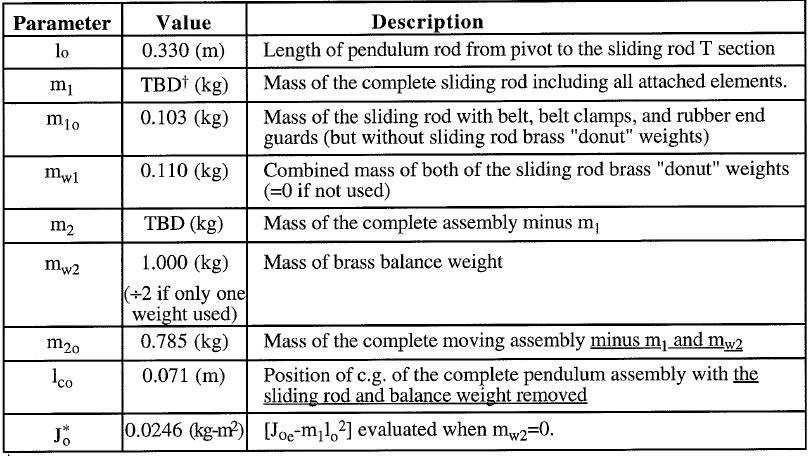
\includegraphics[width = \textwidth]{masspropertyvalues.png}
\caption{Mass Property Values}
\label{Fig4}
\end{figure}
It is necessary to identify pertinent dynamic and scaling parameters in order to design and implement controllers which stabilizes the inverted pendulum plant and allows it to track set points in angular displacement. It is recognized that not all parameters may be measured with a fully assembled pendulum.Figure \ref{Fig4} shows the parameters which are fixed. Their nominal values have been measured prior to assembly.$l_{w2}$ is a signed distance from the pivot to the $c_g$ of the balance mass $m_{w2}$. The various distances for the calculation of $l_{w2}$ is shown in figure \ref{Fig5}.From the definitions given in figure \ref{Fig4}, we have:
\begin{equation}\label{eq:23}
m_1 = m_{1o} + m_{w1}
\end{equation}
\begin{equation}\label{eq:24}
m_2 = m_{2o} + m_{w2}
\end{equation}
\begin{equation}\label{eq:25}
l_{w2} = -\frac{t + l_t + l_b}{2}
\end{equation}
\begin{equation}\label{eq:26}
l_c = \frac{m_{w2}l_{w2} + m_{2o}l_{co}}{m_2}
\end{equation}
\begin{equation}\label{eq:27}
J_{oe} = J^* + m_1l_0^2 + m_{w2}l_{w2}^2
\end{equation}
\begin{figure}[H]
\centering
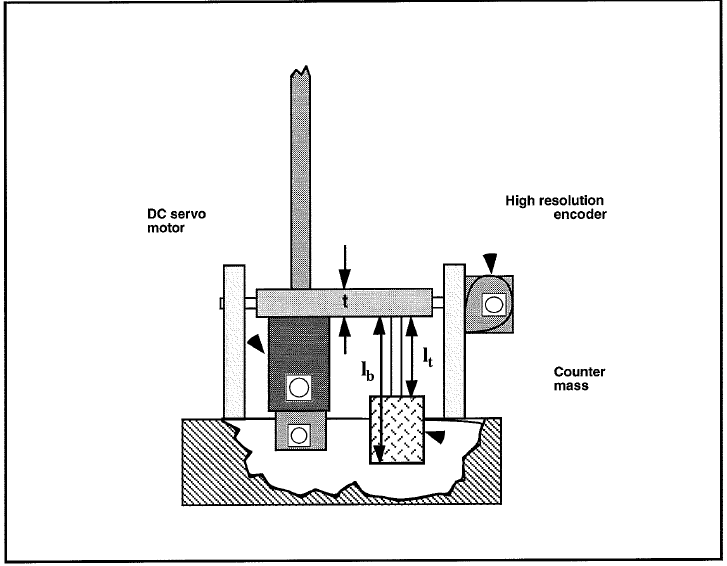
\includegraphics[width = \textwidth]{lw2.png}
\caption{Lengths for $l_{w2}$ Calculations}
\label{Fig5}
\end{figure}
For calculating $J^*$, we remove the brass mass. Hence the equation reduces to \eqref{eq:29}
\subsection{Procedure For obtaining Hardware Gain}
\begin{figure}[H]
\centering
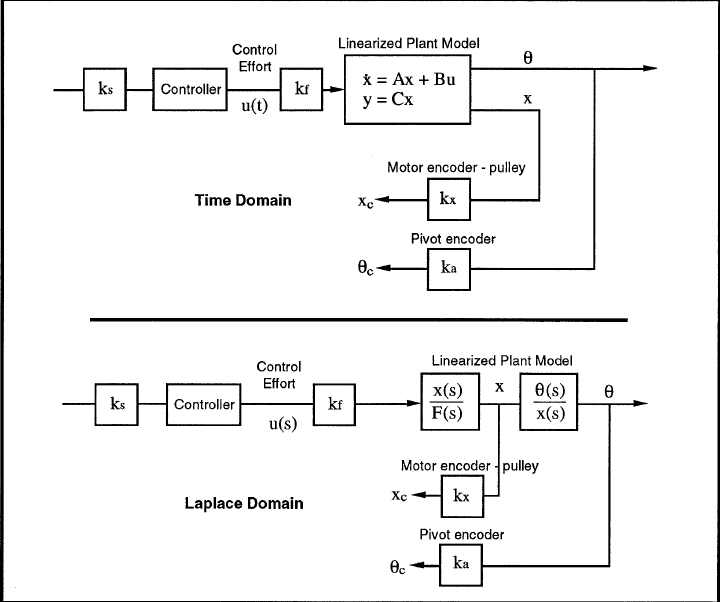
\includegraphics[width = \textwidth]{kakx.png}
\caption{Plant block diagram with scale factors}
\label{Fig6}
\end{figure}
To find hardware gain, the values of $k_a$ and $k_x$ should be confirmed. These are scale factors. The procedure to find these values of the scale factors are as follows:
\begin{enumerate}
\item Remove power cord from the control box, but have all other cables connected.
\item Position the pendulum rod to the right and the sliding rod to the far right of the limit travel.
\item Select Zero Position from the Utility menu. Now the position of Encoder1 and Encoder2 will be zero in the display.
\item Hold on to the pendulum rod and push the sliding rod from one end until it hits the opposite end of its travel. Note the count of the Encoder2 on the screen.
\item Calculate the distance traveled by the sliding rod in meters. The ratio of the two is the value of $k_x$.
\item Move pendulum rod in the anticlockwise direction all the way to left.
\item Record the number of counts on Encoder1. Measure the angle moved by the pendulum in radians. The ratio of the two values gives $k_a$.
\end{enumerate}
\textbf{Result} The value of scale factors are given in the figure \ref{Fig7}
\begin{figure}[H]
\centering
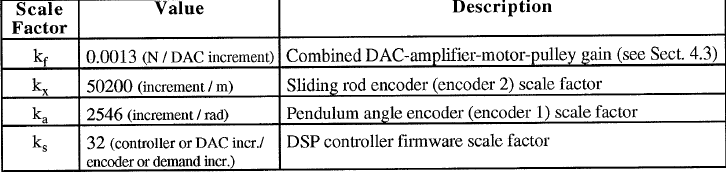
\includegraphics[width = \textwidth]{kxkavalues.png}
\caption{Scale Factor Confirmation Values}
\label{Fig7}
\end{figure}
\subsubsection{Procedure to Confirm $J_{oe}$}
\begin{enumerate}
\item Remove the Brass balance weights from the apparatus and install both donut weights on the sliding rod.
\item Use a rubber band to restrain the sliding rod in the center of travel as shown in figure \ref{Fig8}
\item Disconnect power cord from the control box but leave the other cables connected
\item Very carefully position the entire pendulum mechanism upside down, so that the system can be operated in a normal pendulum mode.Keep the assembly supported between the edges of the table. Now pendulum is hanging freely
\item With controller powered up, from the interface click Set-Up menu $\rightarrow$ Control Algorithm $\rightarrow$ set Ts= 0.0044s $\rightarrow$ OK.
\item Go to Data$\rightarrow$ Setup Data Acquisition$\rightarrow$select Encoder1 as data to be acquired and Data Sampling 5 servo cycles (5Ts)$\rightarrow$OK to exit Setup Data Acquisition$\rightarrow$select Encoder1 as data to be acquired and Data Sampling 5 servo cycles (5Ts)$\rightarrow$OK to exit.
\item Go to Utility$\rightarrow$Zero Position. This make the encoder position as zero.
\item Go to Command$\rightarrow$Trajectory$\rightarrow$Step dialog box$\rightarrow$ step-up$\rightarrow$Open-loop Step, Step size=0, Duration=10000 ms, repitition-1 $\rightarrow$The data will be acquired for 20 s by the controller but without driving the actuator.
\item Go to Command$\rightarrow$Execute and then manually disturb the pendulum
\item Ones the data is collected, a dialog box will be opened. click OK
\item Go to Plotting$\rightarrow$Setup Plot$\rightarrow$choose Encoder-1 position
\item Goto Plotting$\rightarrow$Plot Data
\end{enumerate}
\begin{figure}[H]
\centering
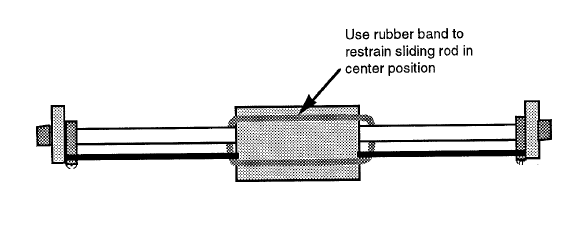
\includegraphics[width = \textwidth]{rubberband.png}
\caption{How to restrain sliding rod in the center using the rubber band}
\label{Fig8}
\end{figure}
\textbf{Calculation} From the oscillation of the normal pendulum, find the time period T. Use \eqref{eq:28} to find $J_{oe}$.
\begin{equation}\label{eq:28}
J_{oe} = ml_{cg}g\Bigg(\frac{T}{2\pi}\Bigg)^2
\end{equation}
where, m is the total mass of the system without brass weights,  m=0.998kg and $l_{cg} = 0.126$ For this system, $J^*$ can be found using equation.
\begin{equation}\label{eq:29}
J^* = J_{oe} - m_1l_0^2
\end{equation}
\textbf{Result} The oscillations of the normal pendulum are shown in Figure \ref{Fig9}
\begin{figure}[H]
\centering
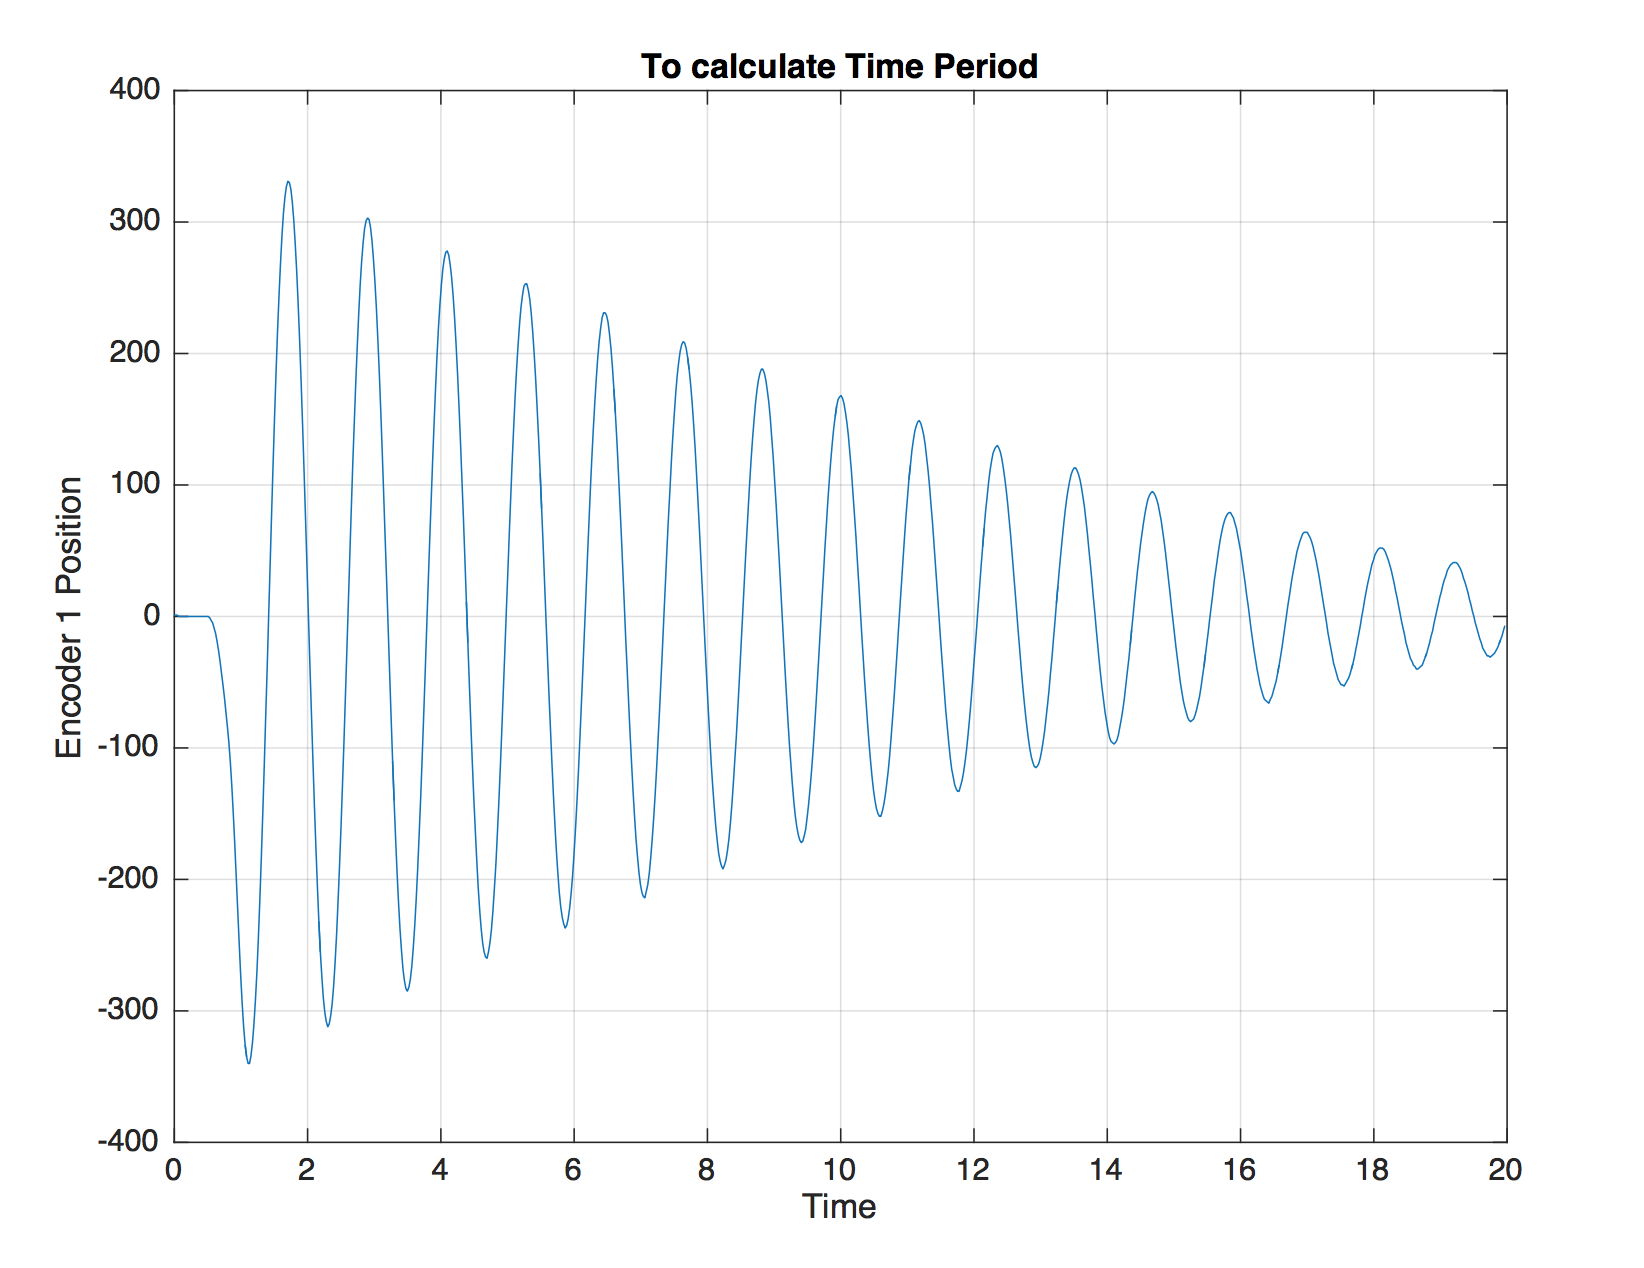
\includegraphics[width = \textwidth]{time.png}
\caption{Normal Pendulum Oscillation}
\label{Fig9}
\end{figure}
$J_{oe} = 0.0478kgm^2$ and $J^* =  0.0246kgm^2$
\subsection{Procedure to Design PD Controller}
\begin{figure}[H]
\centering
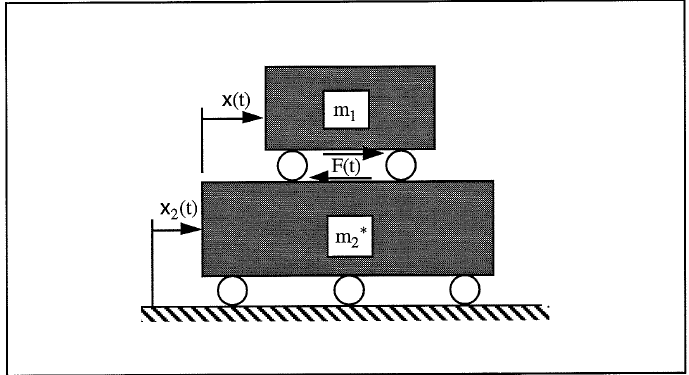
\includegraphics[width = \textwidth]{equivalentmass.png}
\caption{Simplified Model of Sliding Rod Dynamics When Plant is at Equillibrium}
\label{Fig10}
\end{figure}
A simplified dynamic model of the relationship between the sliding rod and the applied force F when the plant is at the equilibrium is shown in \ref{Fig10}. Here the inertia of the pendulum assembly is shown as an equivalent mass $m_2^*$ at the sliding rod interface according to \eqref{eq:30}. To design the controller to the sliding rod, we consider rod assembly as a point mass m* so that the fourth order equation in 20 can be reduced to a second order equation. Now, when the rod is considered as a point mass, the force equation can be written as equation \eqref{eq:31}.
\begin{equation}\label{eq:30}
m_2^* = \frac{J^*}{l_0^2} 
\end{equation}
\begin{equation}\label{eq:31}
F(t) = m^*\ddot{x}
\end{equation}
The transfer function of the rod assemble reduces to \eqref{eq:32}
\begin{equation}\label{eq:32}
\frac{X_c(s)}{F_c(s)} = \frac{k_{hw}}{m_1^*s^2}
\end{equation}
where
\begin{equation}\label{eq:33}
m^* = \frac{m_1m_2^*}{m_1 + m_2^*}
\end{equation}
\begin{equation}\label{eq:34}
k_{hw} = k_xk_sk_f
\end{equation}
The block diagram of the PD controller is shown in the figure \ref{Fig11}
\begin{figure}[H]
\centering
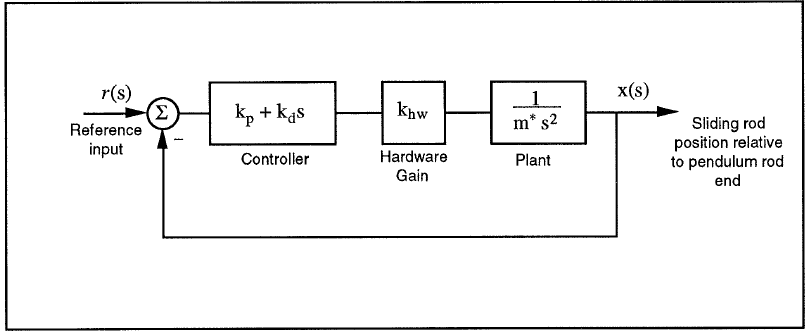
\includegraphics[width = \textwidth]{innerloop.png}
\caption{Block diagram of Rigid Body PID Controller}
\label{Fig11}
\end{figure}
The equations required to design the controller can be obtained from the following equations \eqref{eq:35} to \eqref{eq:38}
\begin{equation}\label{eq:35}
C(s) = \frac{x(s)}{r(s)} = \frac{\frac{k_{hw}}{m_1^*}(k_ds + k_p)}{s^2 + \frac{k_{hw}}{m_1^*}(k_ds + k_p)}
\end{equation}
\begin{equation}\label{eq:36}
\omega_n = \sqrt{\frac{k_pk_{hw}}{m^*}}
\end{equation}
\begin{equation}\label{eq:37}
\zeta = \frac{k_dk_{hw}}{2\sqrt{m^*k_pk_{hw}}}
\end{equation}
\begin{equation}\label{eq:38}
C(s) = \frac{2\zeta\omega_ns + \omega_n^2}{s^2 + 2\zeta\omega_ns + \omega_n^2}
\end{equation}
$\omega_n$ and $\zeta$ are the natural frequency and the damping ratios respectively. The acceptable range of values for $k_p$ and $k_d$ are $0.15 \leq k_p \leq 0.35$ and $0.004 \leq k_d \leq 0.012$
\subsubsection{Procedure for Implementing PID control}
By adjusting the knob above the rod, bring the pendulum to zero position. Please note to turn off the control switch before touching the pendulum. After finding the values for the controller gains, the following method may be followed to assign the values to the same using the Executive Program.
\begin{enumerate}
\item Goto Data $\rightarrow$ Setup Data Acquisition$\rightarrow$ Selected Item [CommandedPosition, Encode-2Position] and Sample Period=2 $\rightarrow$ OK
\item Command $\rightarrow$ Trajectory $\rightarrow$ Setup $\rightarrow$ select Closed loop step, Step size=1000 counts, DwellTime=1000 ms, Repetition=1 $\rightarrow$ OK
\item Setup $\rightarrow$ Setup Control Algorithm $\rightarrow$ Continuous Time Control, Ts=0.00442s $\rightarrow$ PID $\rightarrow$ Setup Algorithm $\rightarrow$ Enter $K_p, K_d$ values, select Encoder2 $\rightarrow$ Implement Algorithm $\rightarrow$ OK
\item Utility $\rightarrow$ Zero Position
\item Turn on the control box
\item Command $\rightarrow$ Execute $\rightarrow$ Run
\item Plot the data i.e. Encoder-2 Output and the Commanded Position, from plot menu
\end{enumerate}
\textbf{Result} This section include the results for the response of the rod assembly. The result that was obtained from the system as well as the ones simulated using MATLAB are included. Cases for Under-damped, critically damped and over-damped are shown.
\begin{figure}[H]
\centering
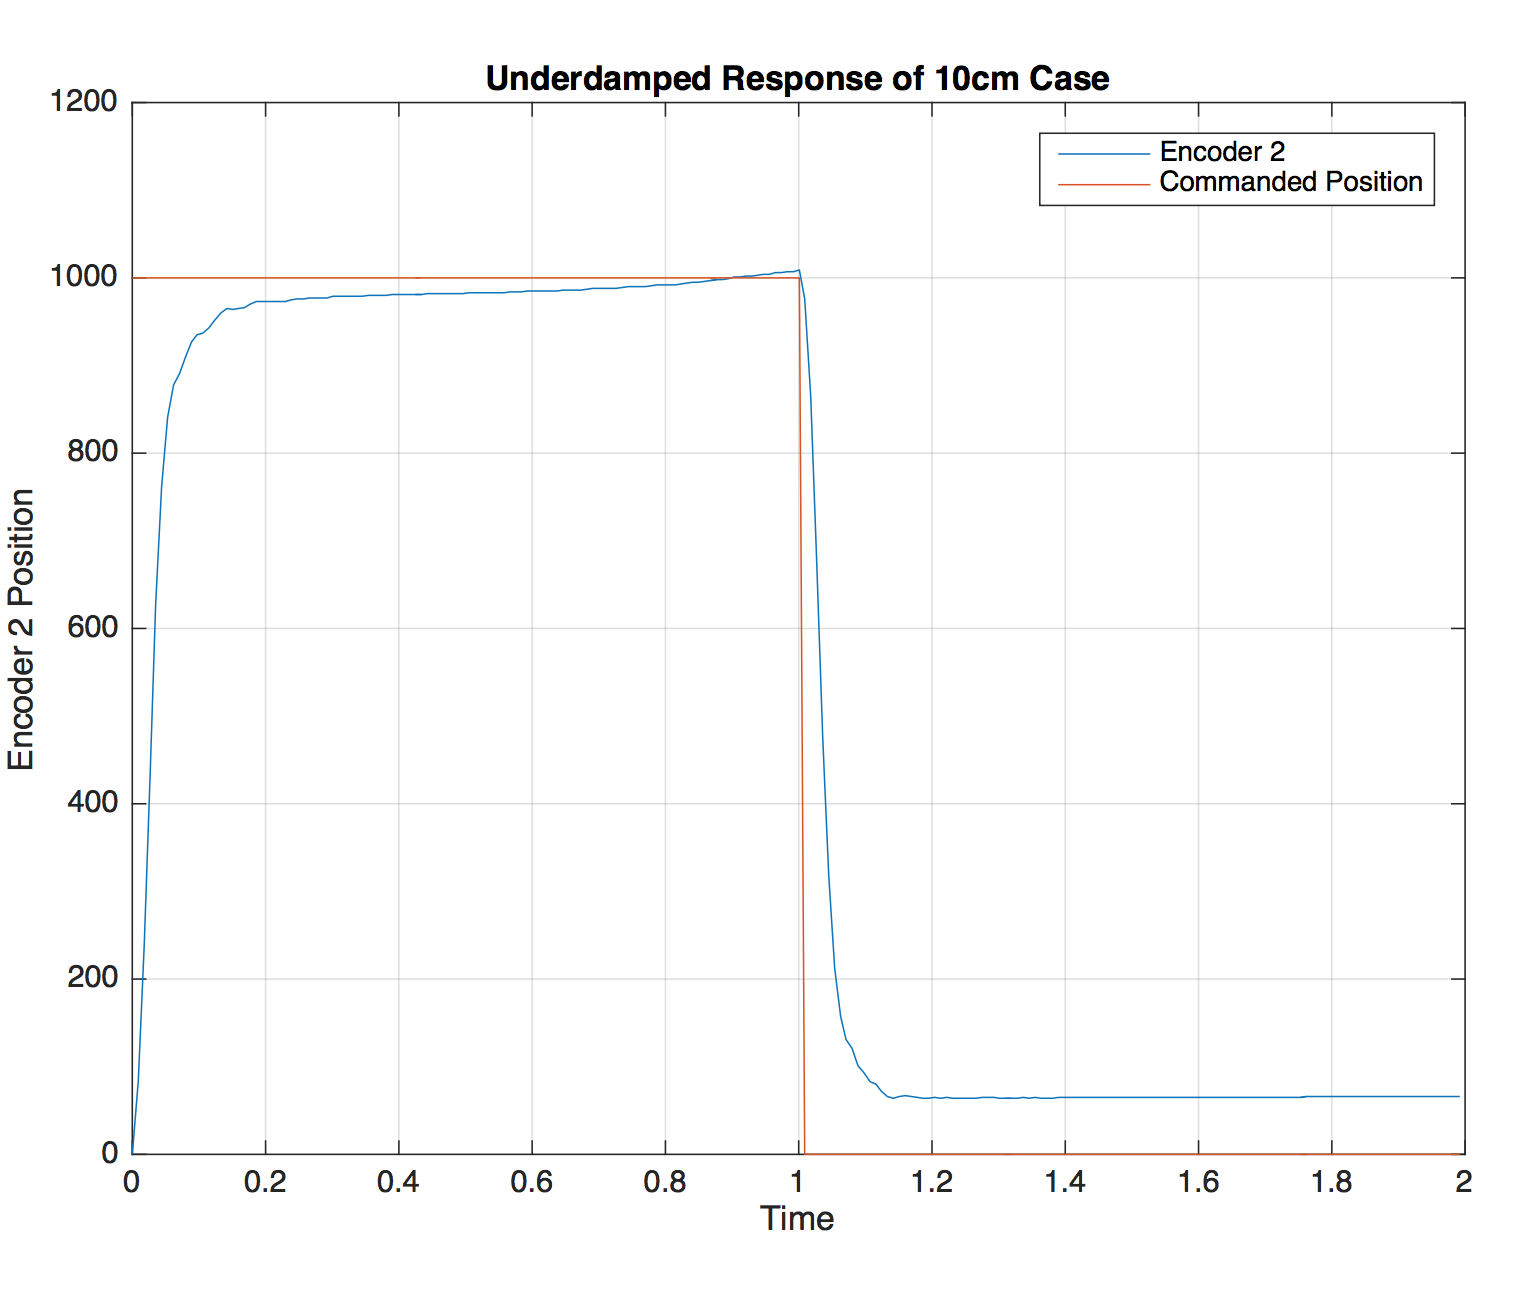
\includegraphics[width = \textwidth]{ud_m1.png}
\end{figure}
\begin{figure}[H]
\centering
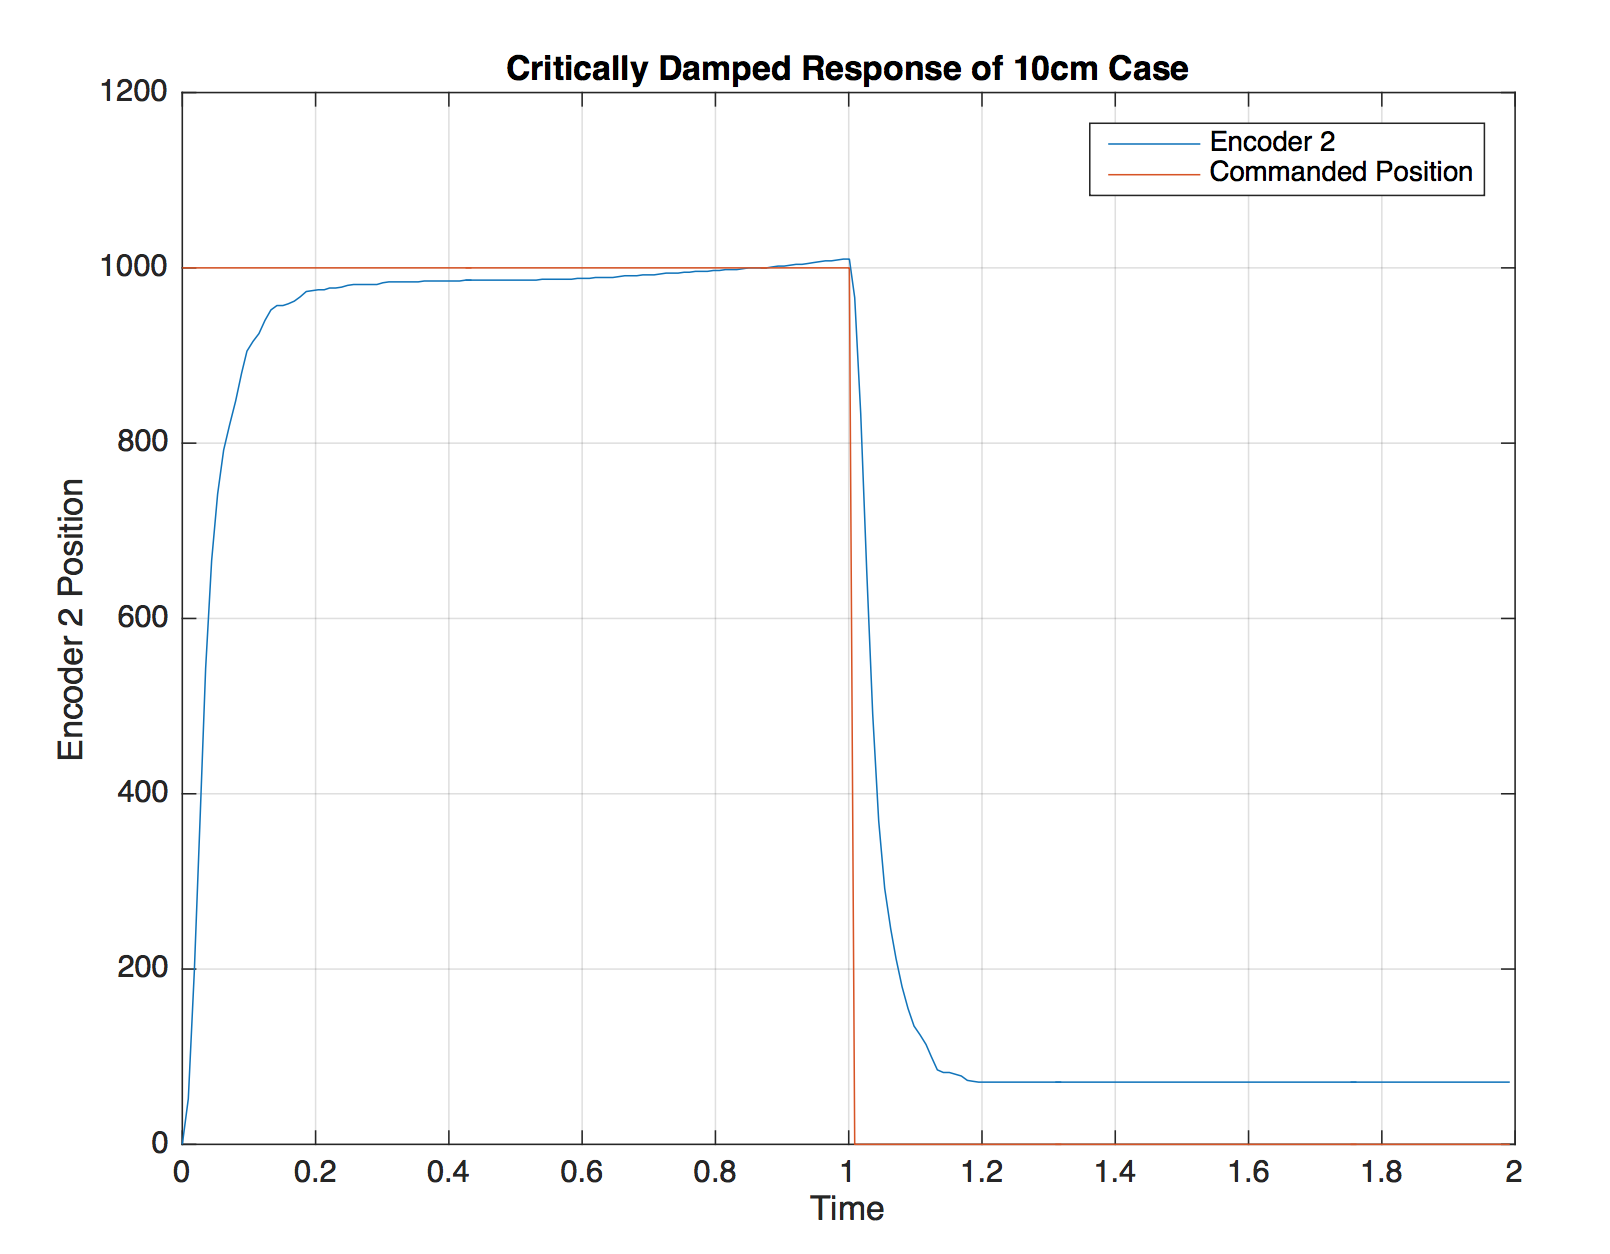
\includegraphics[width = \textwidth]{cd_m1.png}
\end{figure}
\begin{figure}[H]
\centering
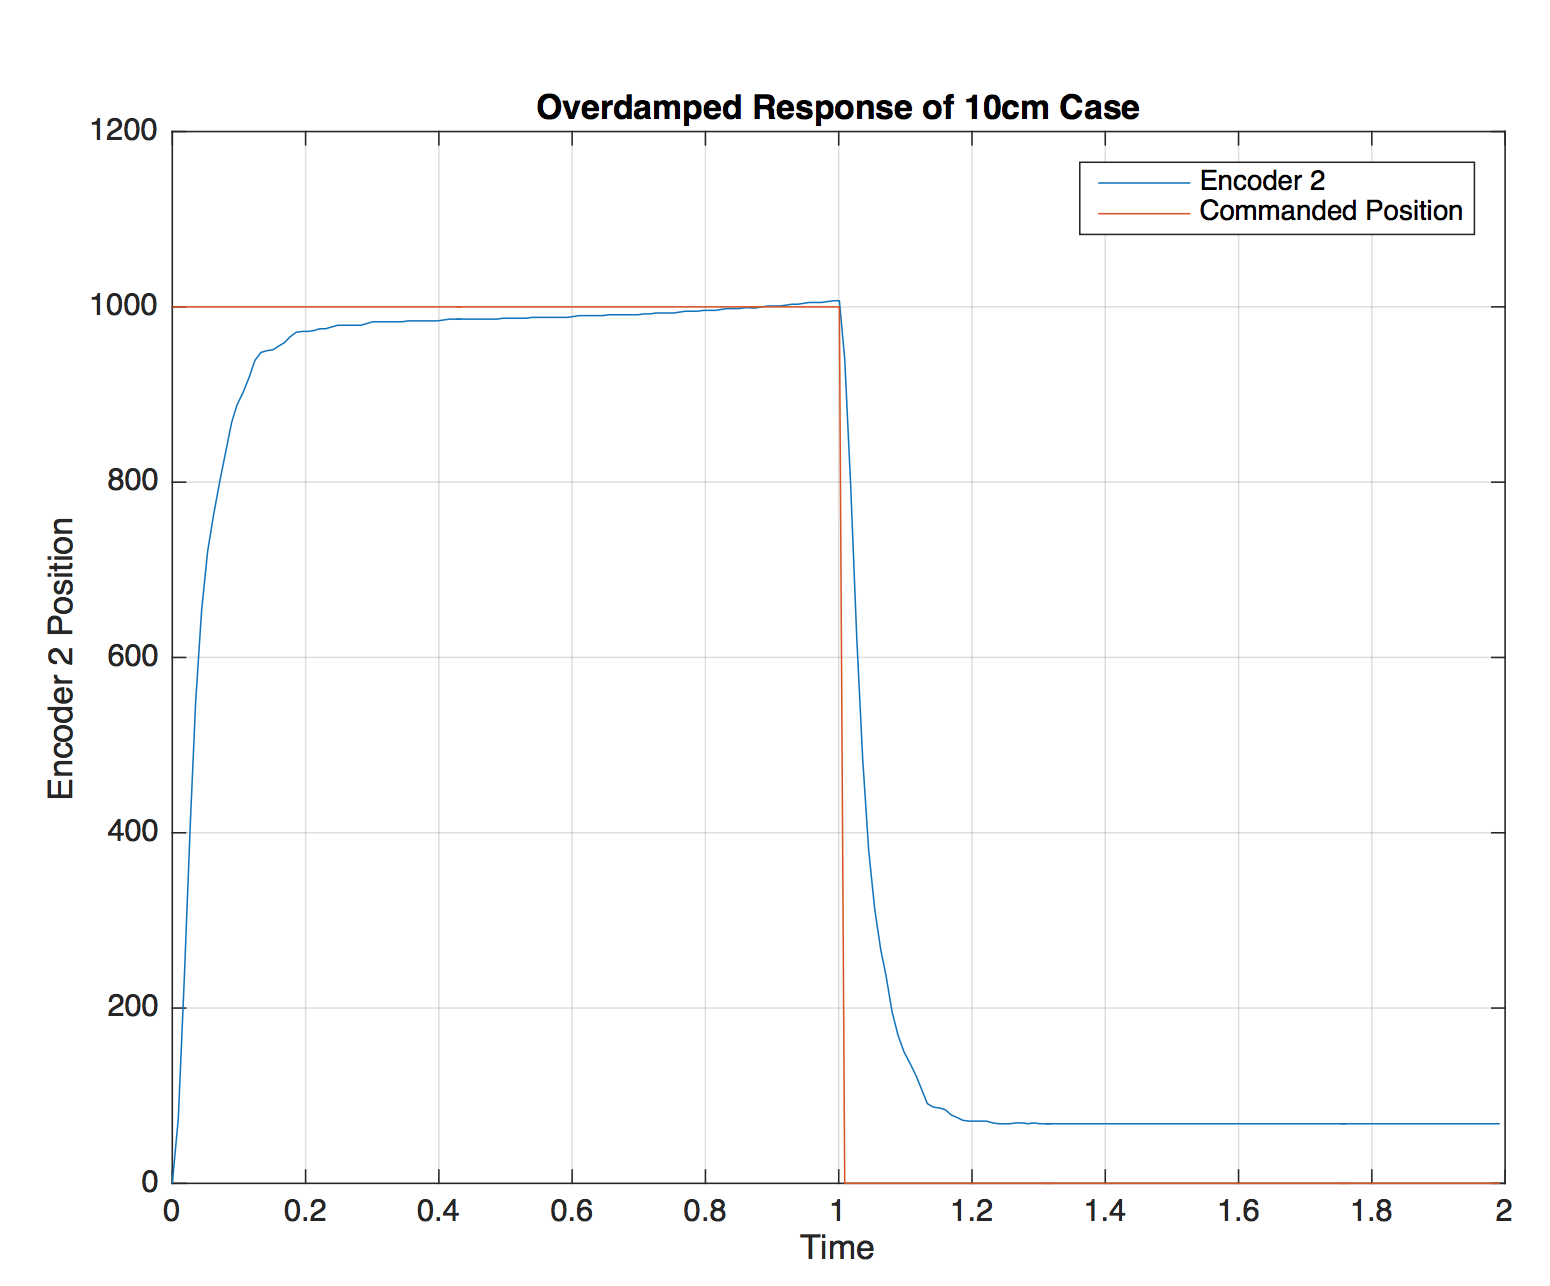
\includegraphics[width = \textwidth]{od_m1.png}
\end{figure}
\begin{figure}[H]
\centering
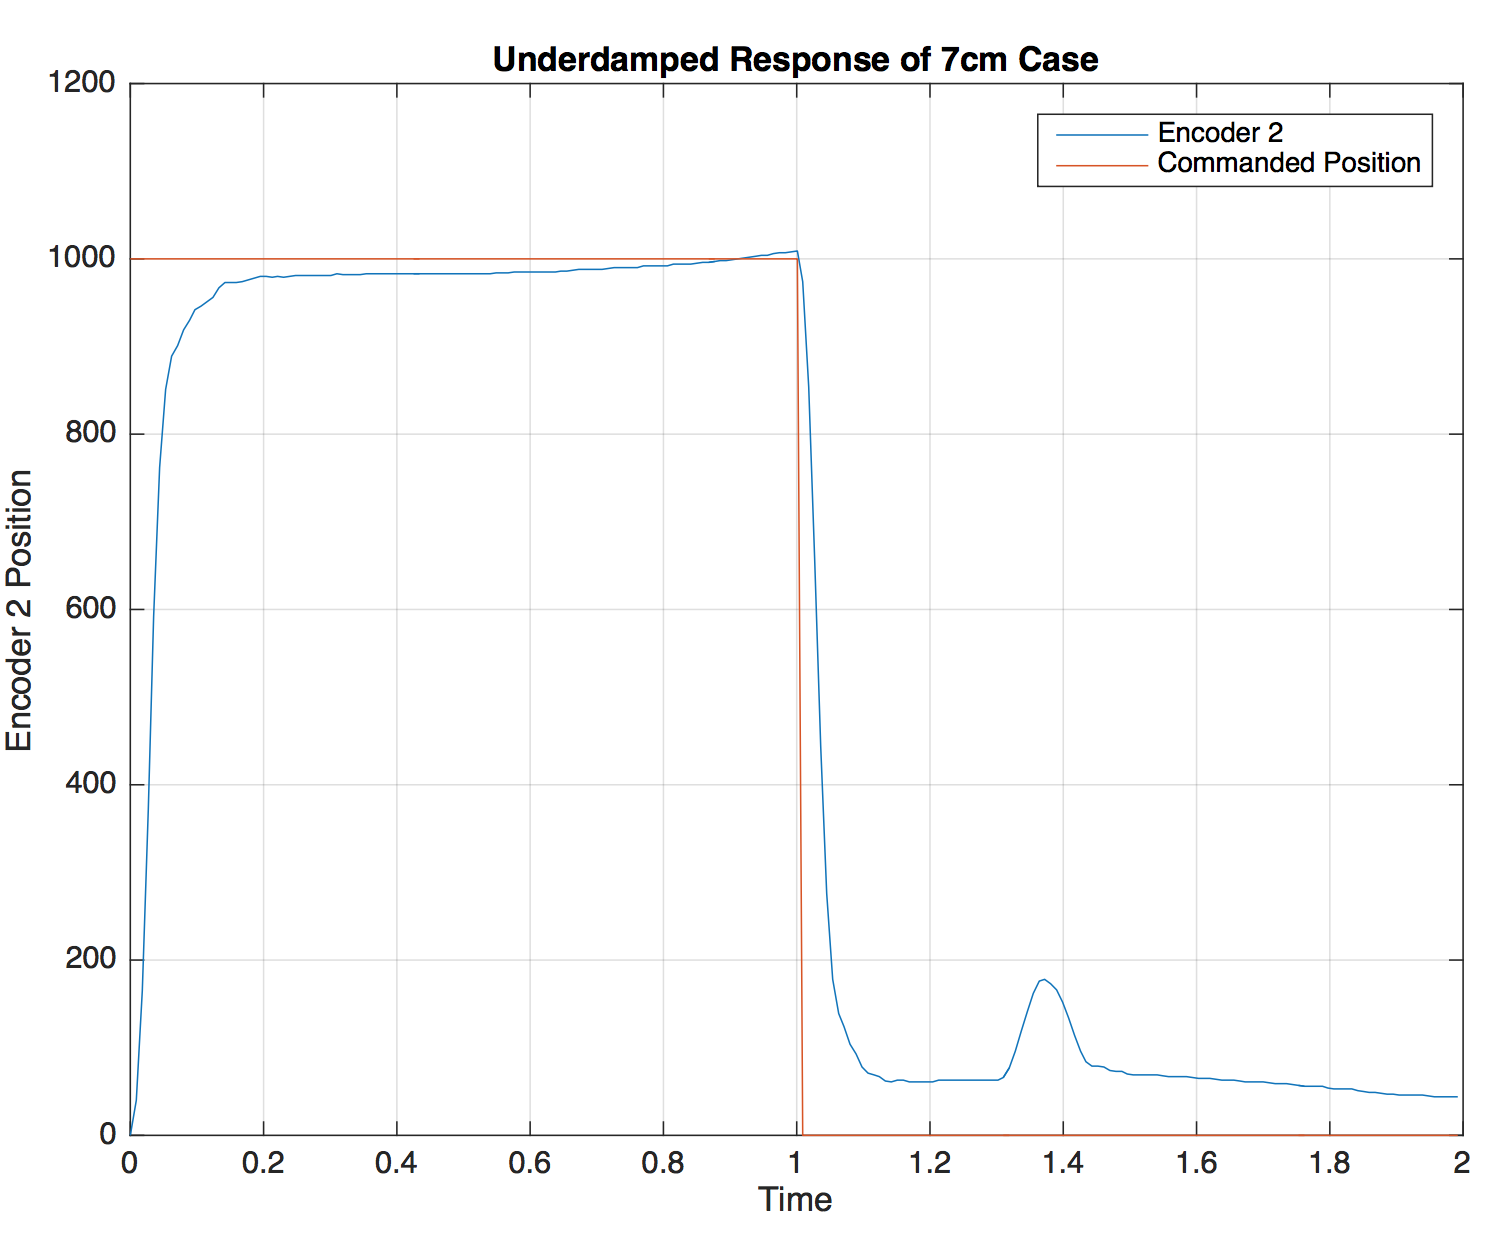
\includegraphics[width = \textwidth]{ud_m2.png}
\end{figure}
\begin{figure}[H]
\centering
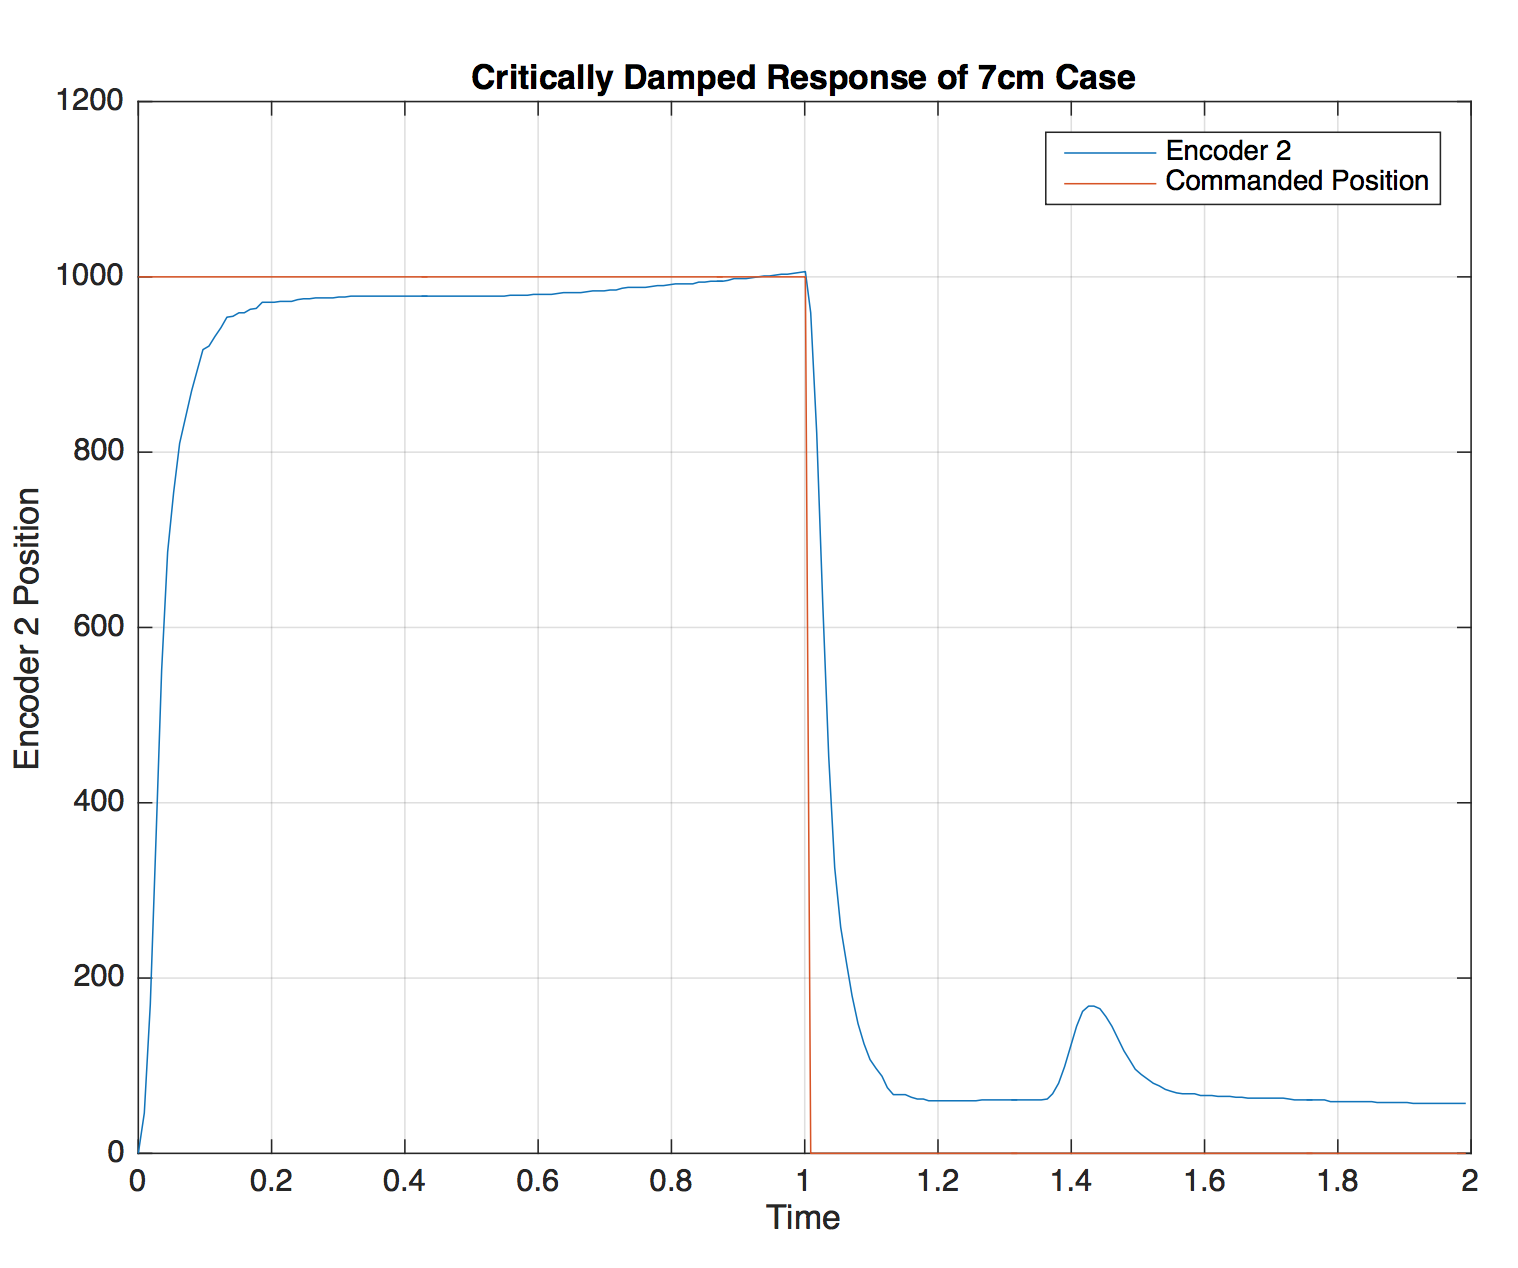
\includegraphics[width = \textwidth]{cd_m2.png}
\end{figure}
\begin{figure}[H]
\centering
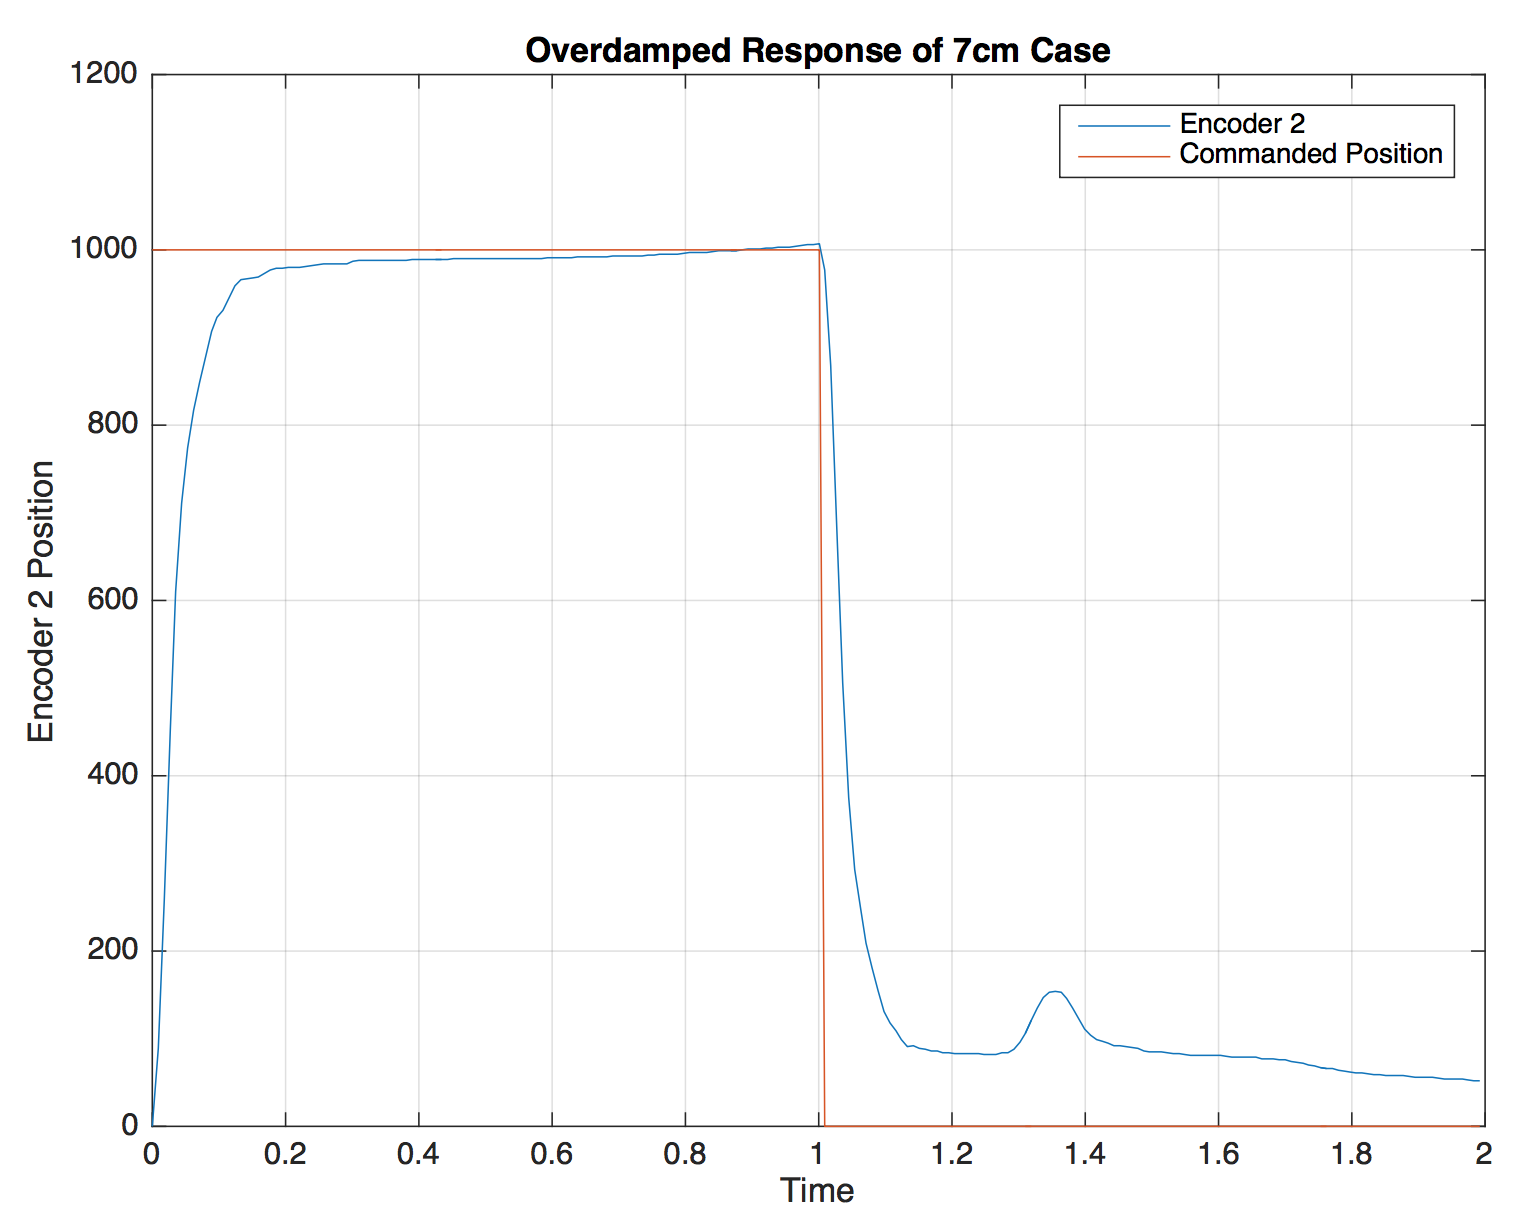
\includegraphics[width = \textwidth]{od_m2.png}
\end{figure}
\end{document}